\documentclass[peerreview]{IEEEtran}
\usepackage{cite} % Tidies up citation numbers.
\usepackage{url} % Provides better formatting of URLs.
\usepackage[utf8]{inputenc} % Allows Turkish characters.
\usepackage{booktabs} % Allows the use of \toprule, \midrule and \bottomrule in tables for horizontal lines
\usepackage{graphicx}
\usepackage{xcolor}

\usepackage{listings}
\usepackage{hyperref}

\definecolor{mygreen}{rgb}{0,0.6,0}
\definecolor{mygray}{rgb}{0.5,0.5,0.5}
\definecolor{mymauve}{rgb}{0.58,0,0.82}

\lstdefinestyle{CStyle}{
  belowcaptionskip=1\baselineskip,
  breaklines=true,
  frame=L,
  xleftmargin=\parindent,
  language=C,
  showstringspaces=false,
  basicstyle=\footnotesize\ttfamily,
  keywordstyle=\bfseries\color{green!40!black},
  commentstyle=\itshape\color{purple!40!black},
  identifierstyle=\color{blue},
  stringstyle=\color{orange},
}

\hyphenation{op-tical net-works semi-conduc-tor} % Corrects some bad hyphenation 

\begin{document}
%\begin{titlepage}
% paper title
% can use linebreaks \\ within to get better formatting as desired
\title{System on Chip Architecture \\ Lab 3 Report}

% author names and affiliations

\author{Daniele Castro S253244\\
System-on-chip architecture\\
Politecnico of Turin\\
}
\date{26/12/2018}

% make the title area
\maketitle
\tableofcontents
\listoffigures
%\end{titlepage}

\IEEEpeerreviewmaketitle
\begin{abstract}
In this lab I have implemented a simple web server using the MCU STM32F051R8 on the discovery board and the WiFi module SPWF01SX.11 communicating with the microcontroller and using AT commands. Web pages are updated by sending HTML code through UART (RS-232) with TTL voltage levels.
\end{abstract}
\section{Introduction}
During the development of this lab I have met some issues regarding both the code structure and even its behaviour. At first I thought to simply go ahead in the development of my custom commands but, then, I decided to fix, some misbehaviour. Maybe it can be useful to someone in the future.
\section{Background}
The SPWF01SX.11 module is a MCU itself with his own firmware. So, to make this laboratory faster,  it would be better to program the module itself instead of making a communication using the serial UART or SPI port to send commands from the STM32 to the module. Anyway, nowdays these kind of modules are going to be very popular because developing an IOT embedded system is really easy with these modules. We can really control a lot of features with its AT commands such as its ADC peripheral.
\section{Proposed Solution}
The main problem with the behaviour of this template was that the HTML code sent appeared to be corrupted: full of strange non ASCII characters. Such charachters were so many that some browsers (like chrome) did not visualize the retrieved HTML file and downloaded it, like in this picture:
\begin{figure}[!h]
\centering
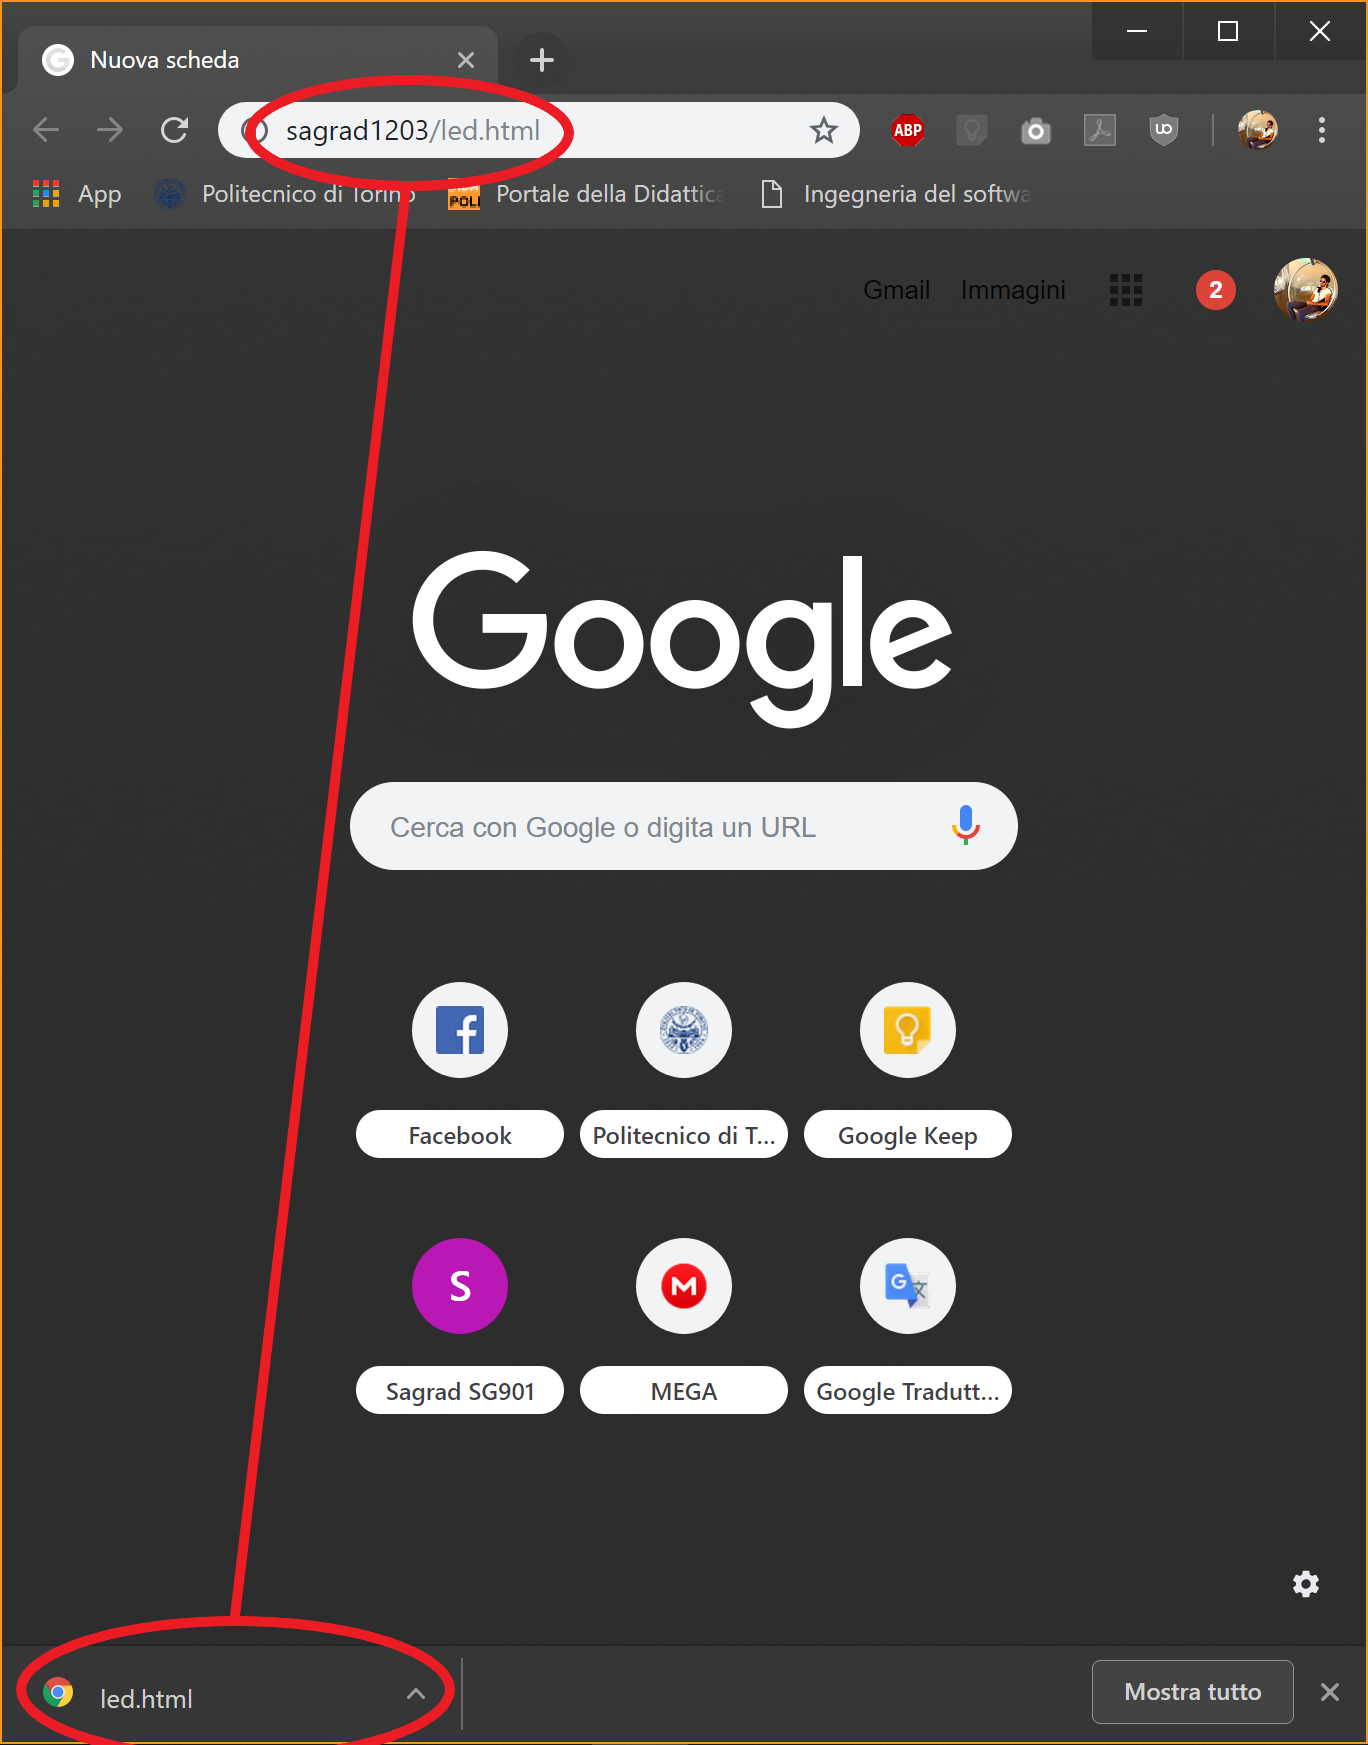
\includegraphics[width=0.45\columnwidth]{7} 
\caption{wrong code download}
\label{fig_download}
\end{figure}
\\while trying to fix this issue I also noticed that HTML web pages were stored in the C code with ASCII characters: in embedded systems they are commonly stored in hexadecimal values so that HTML code can be even stored being formatted without modify any character to store it as a C array. So I decided to rewrite the "led.html" web page with a modern one and to change the storing name from "led.html" to "index.html" so that when we simply write in the browser "http://sagrad1203" we will be automatically redirected to "http://sagrad1203/index.html" (sagrad1203 is the DNS name avoiding to rewrite the IP address that dinamically changes at every reconnection). Anyway, even fixing what showed a strange character was appearing every time at the beginning of every serially uploaded webpage. I discovered that when serially passing the C string:
\begin{lstlisting}[style=CStyle]
uint8_t TxBuffer_Prepare_led_page_upload[] = "at+s.fsa=/index.html,1023\r\n";
\end{lstlisting}
the \lstinline[style=CStyle]{'\r'} was stored at the beginning of every serially passed HTML file (maybe because of a firmware bug of the module). So, I removed that character. As a result I obtained a well displayed web page but If I attached my serial port to the communication bus I saw a bed formatting of the serial AT commands. In any case these commands are not normally shown, so it does not matter. At this point there were only few compilation warnings given by an unexplicited C type casting that I corrected. Other behavioural modifications I have made were in adding the form of cgi\_demo.html in index.html so that I can directly send commands from that web page without hand write cgi\_demo.html. Of course I even had to modify this file because, after test.cgi has been called by the button click, it calls back cgi\_demo.html that, now, contains only a waiting message. After 5 seconds page will be redirected back to index.html. During this time the MCU has enough time to re-upload the index.html with the updated LED status. Now, concerning the "dispall" custom command I have made, I had to send the AT command serially "AT+S.STS=ip\_ipaddr" that, as datasheet explains, would show me the only "ip\_ipaddr" variable. Unfortunally, again maybe because of a firmware bug of the modul, whatever I put after "=" the "AT+S.STS"  showed me the entire variable environment of the module. So I had to post-process the command on the MCU.
\begin{figure}[!h]
\centering
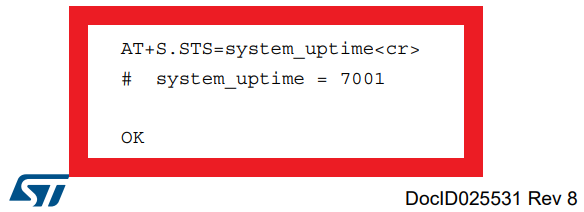
\includegraphics[width=0.51\columnwidth]{6} 
\caption{User Manual screenshot}
\label{fig_datasheet}
\end{figure}
\section{Results and discussion} 
Here are some screenshots I have made to show the final result. On the right there is the serial console showing what is happening on the TX pin of the WiFi module so that we can also see the echo of the AT commands sent from the MCU and the module response but not the HTML code sent because the module does not echo it back during a file transfer. On the left, instead, there is a browser showing the web pages:
\begin{figure}[!h]
\centering
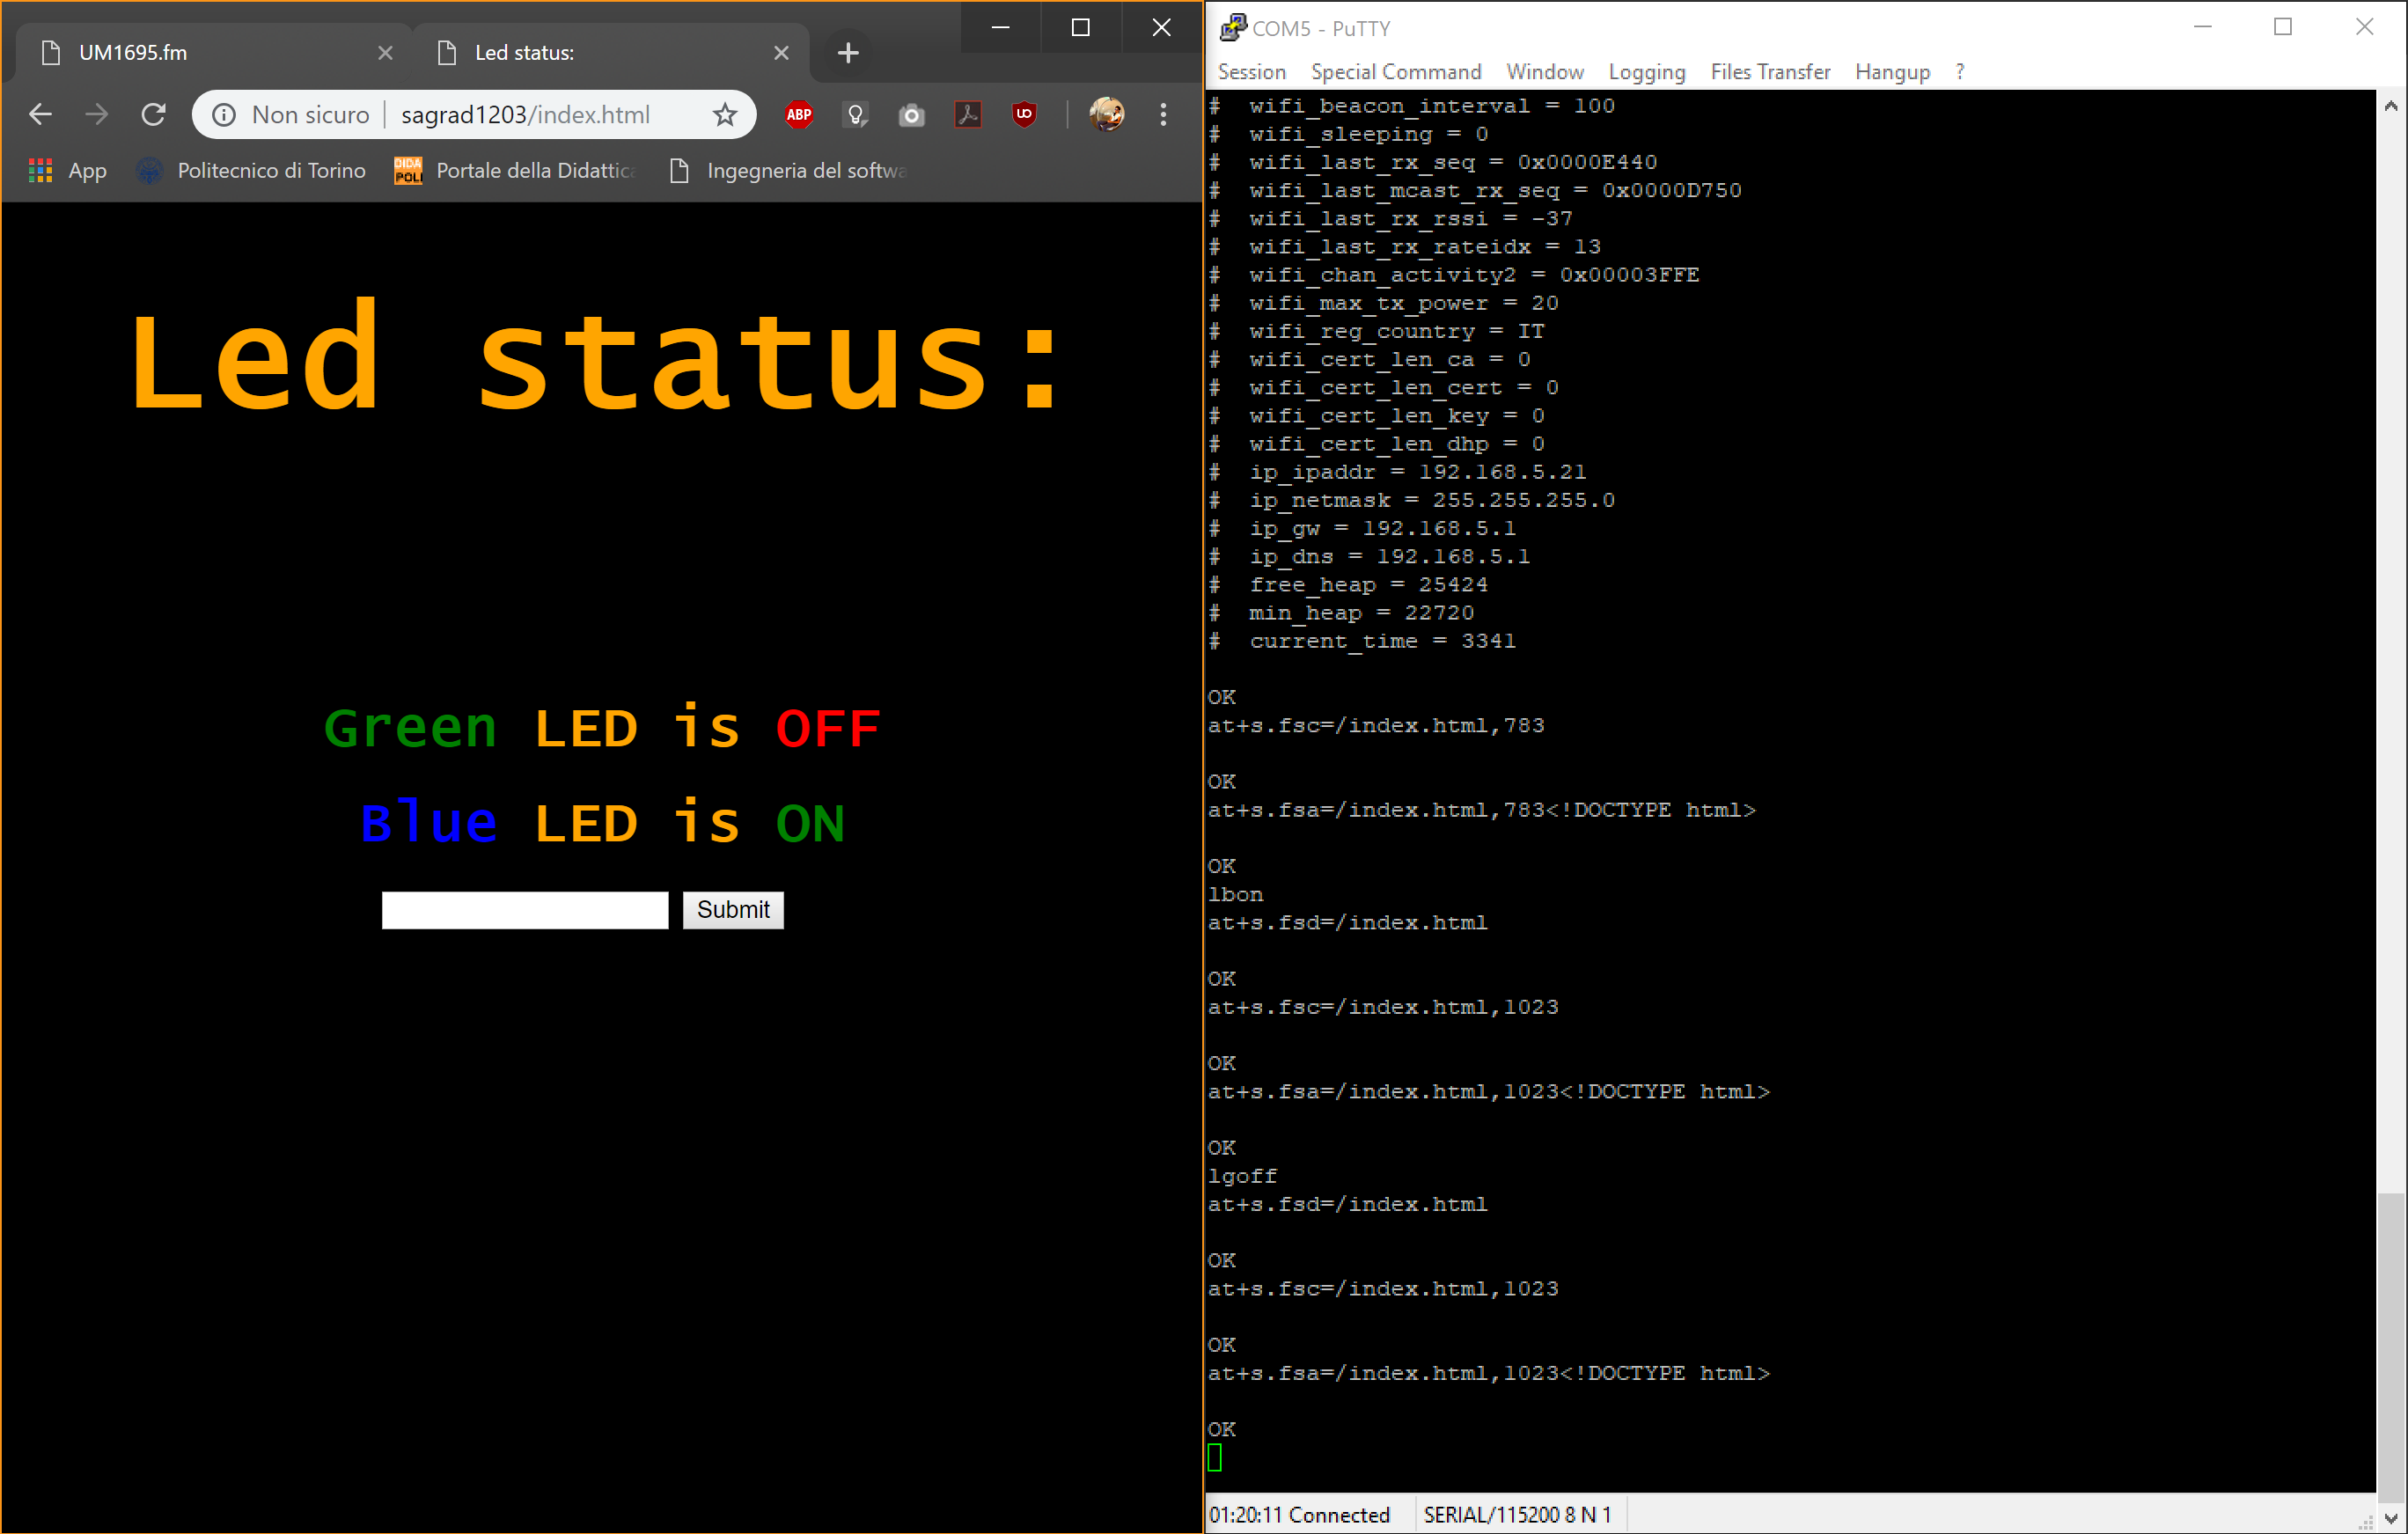
\includegraphics[width=0.8\columnwidth]{1}
\caption{index web page}
\label{fig_index}
\end{figure}
\begin{figure}[!h]
\centering
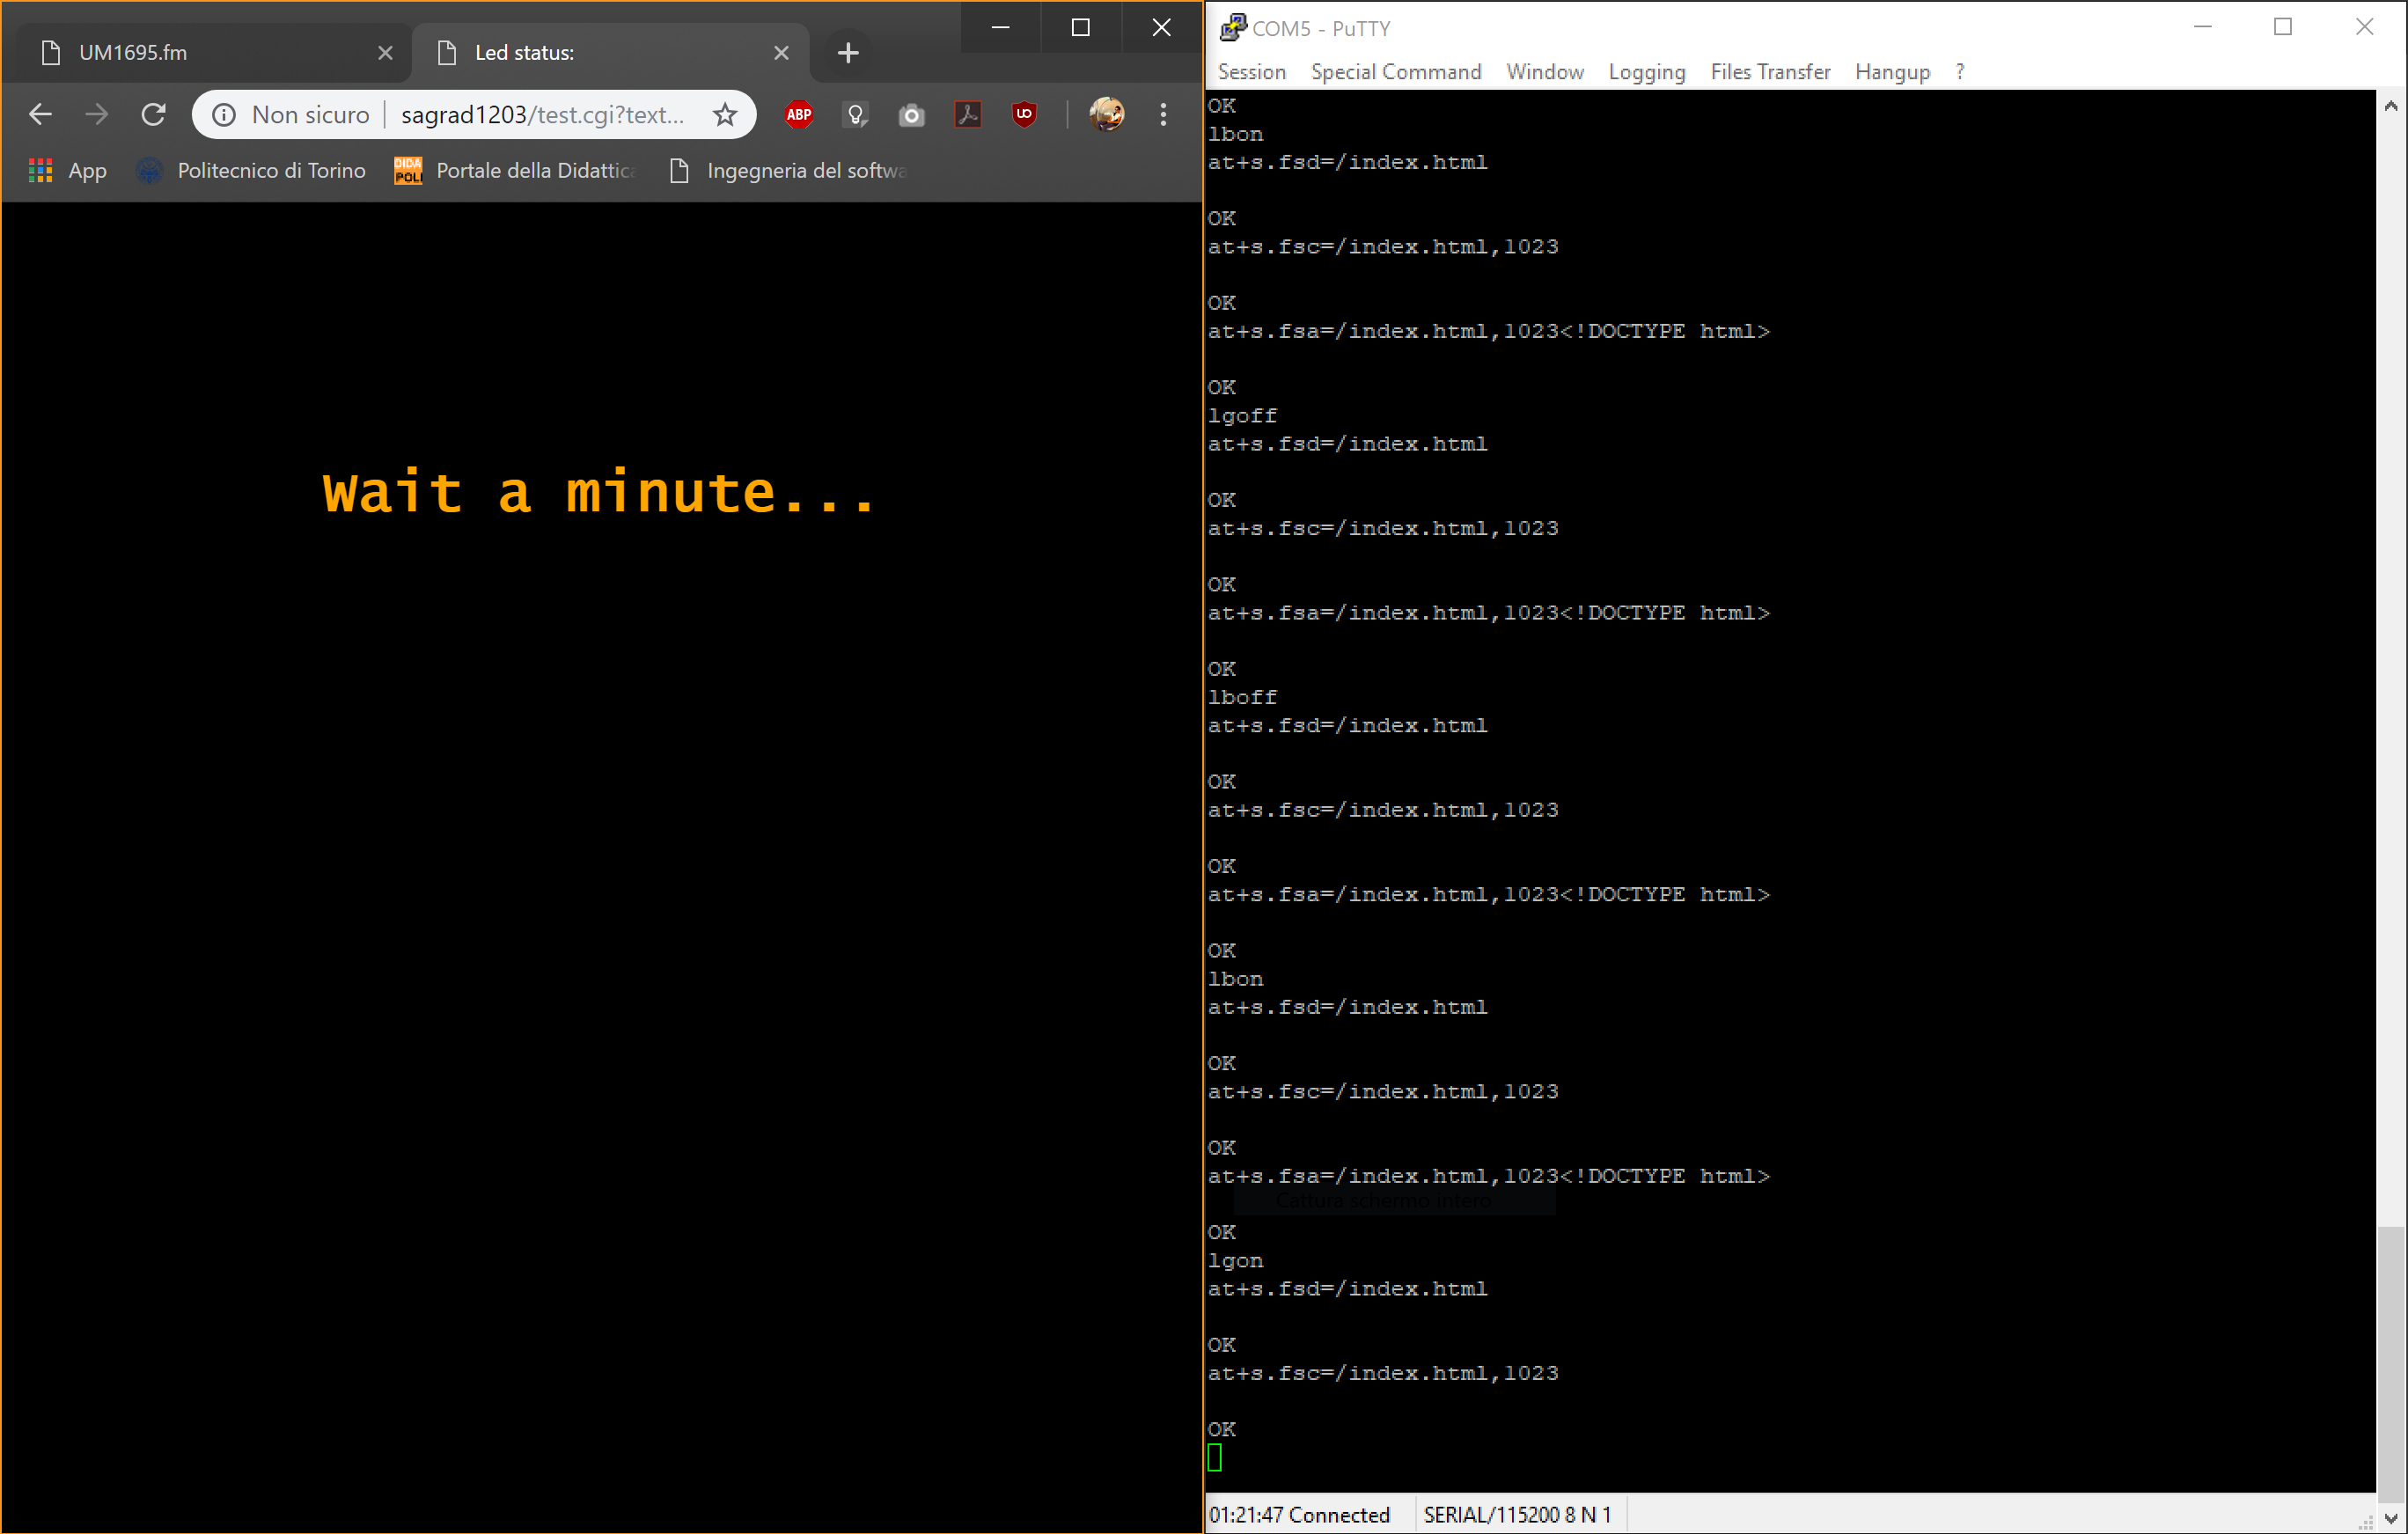
\includegraphics[width=0.8\columnwidth]{2}
\caption{wait web page}
\label{fig_wait}
\end{figure}
\begin{figure}[!h]
\centering
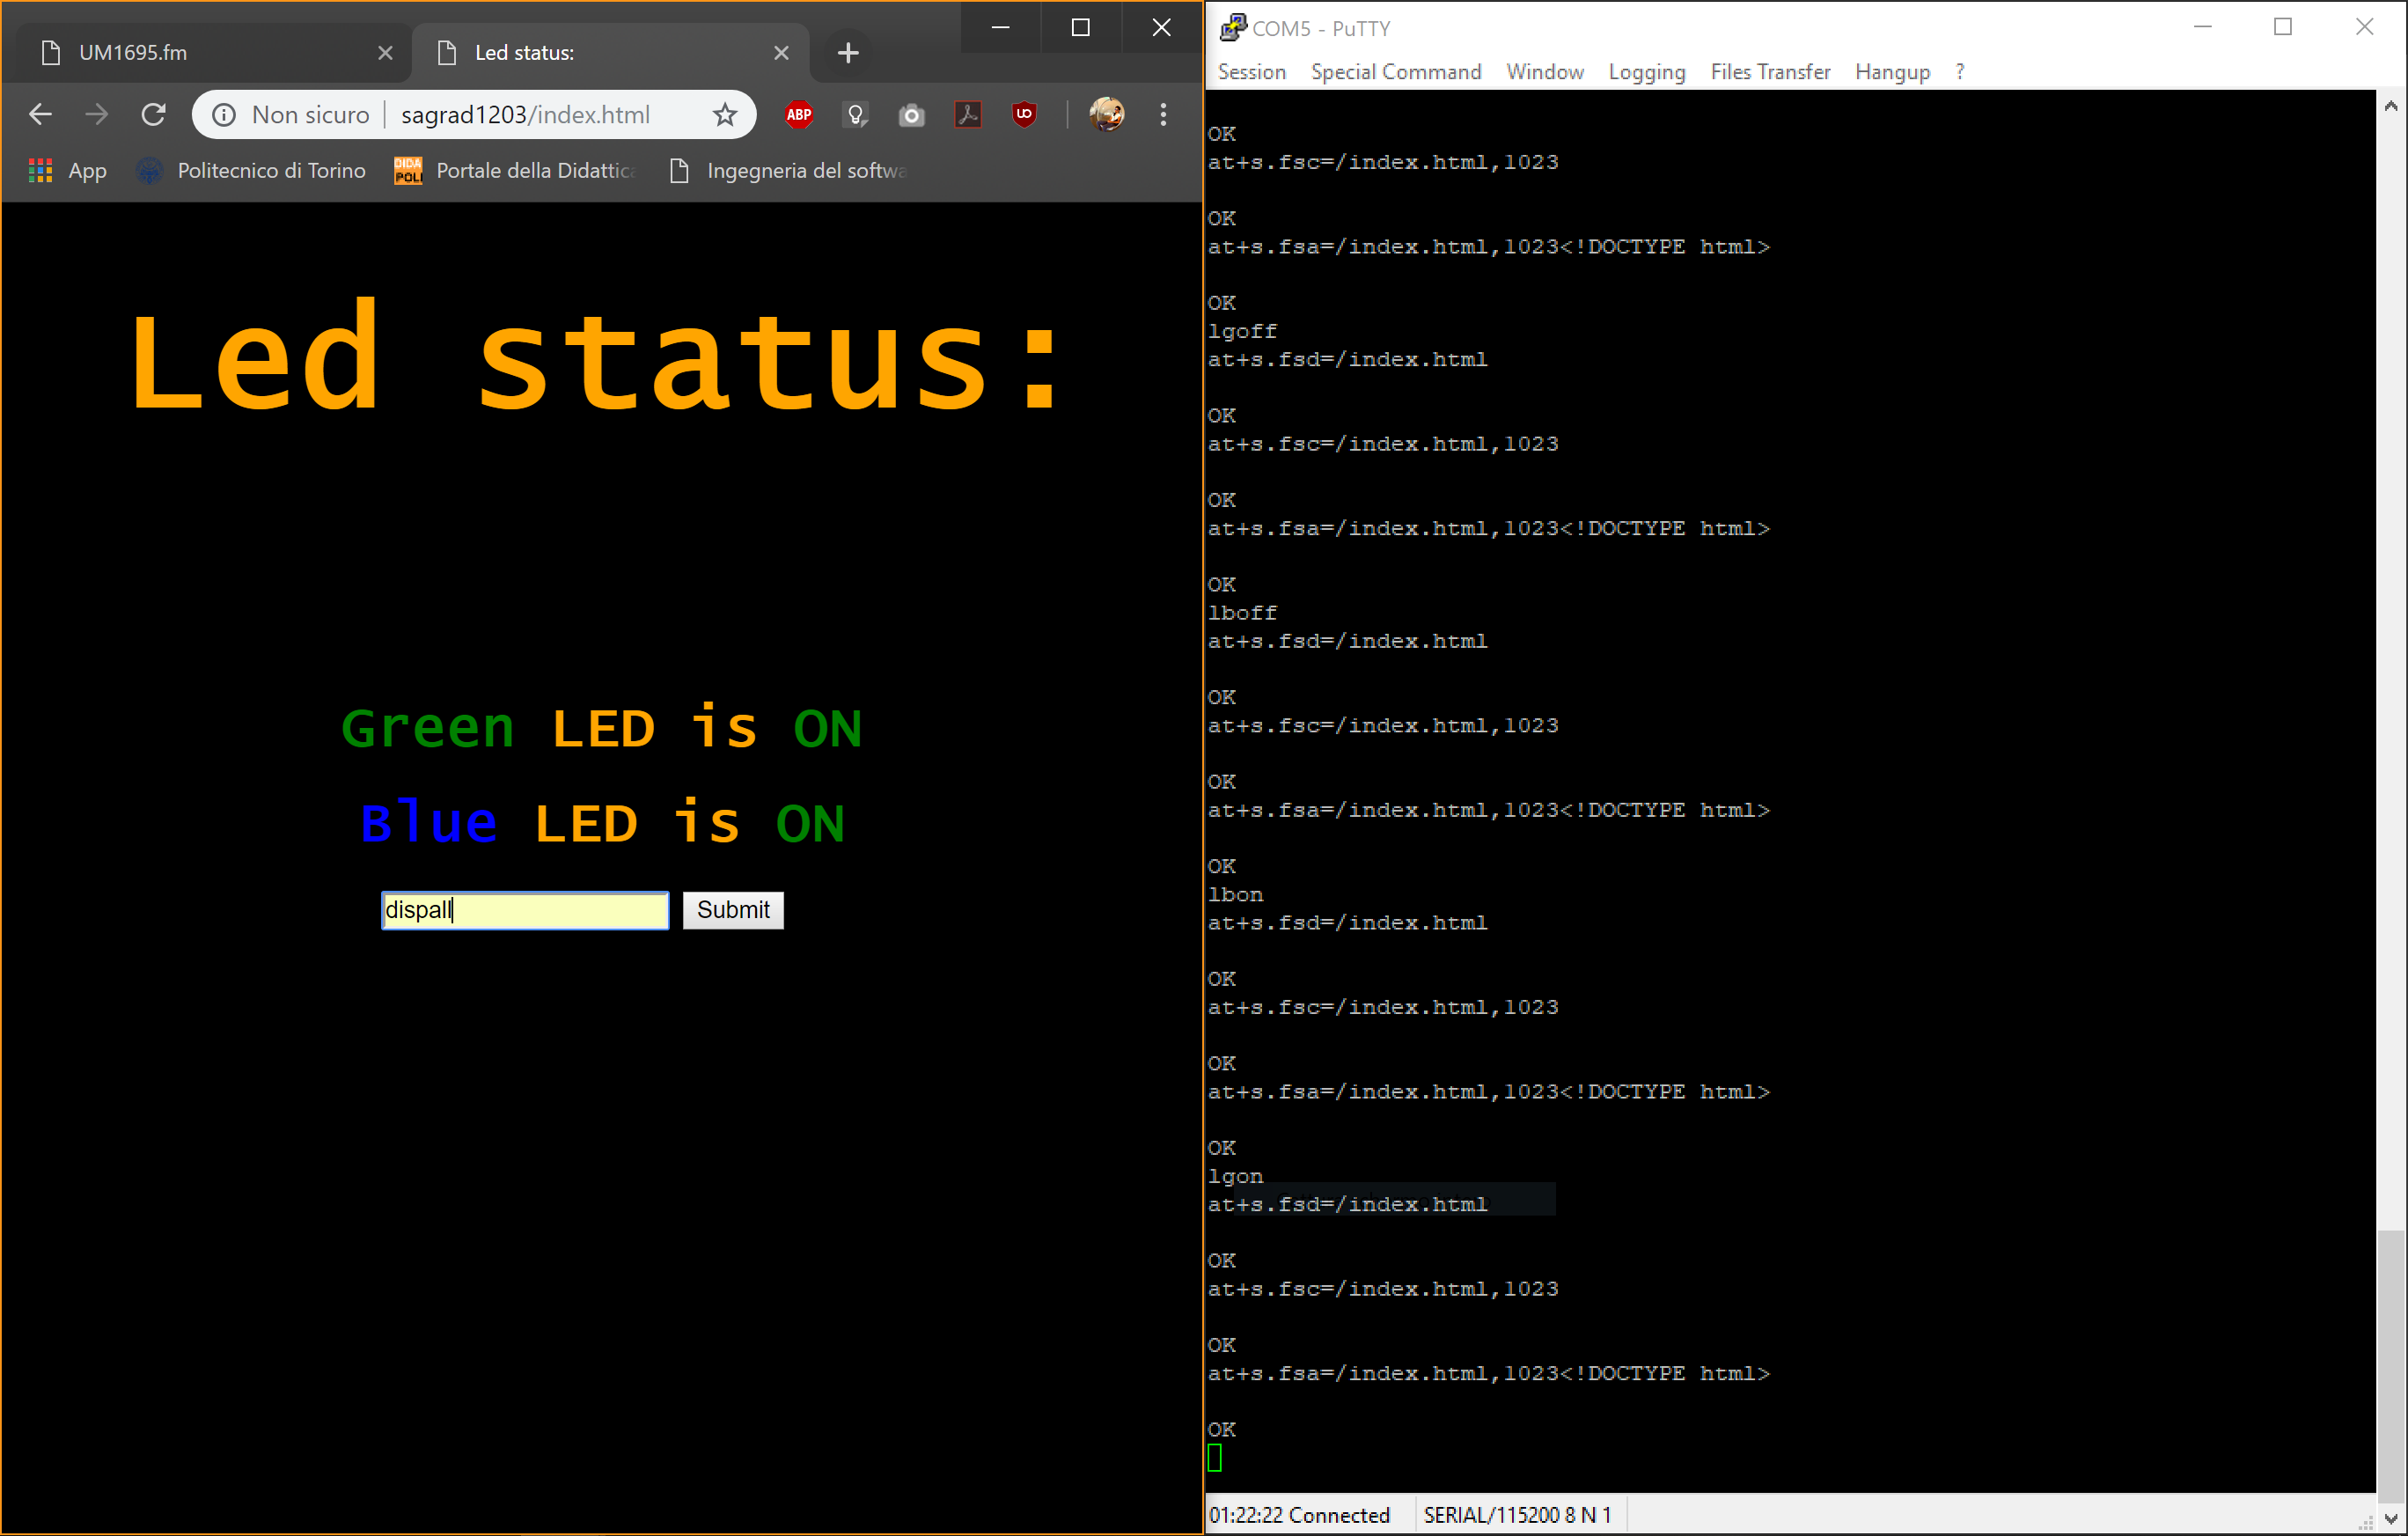
\includegraphics[width=0.8\columnwidth]{3}
\caption{updated index web page}
\label{fig_updated}
\end{figure}
\begin{figure}[!ht]
\centering
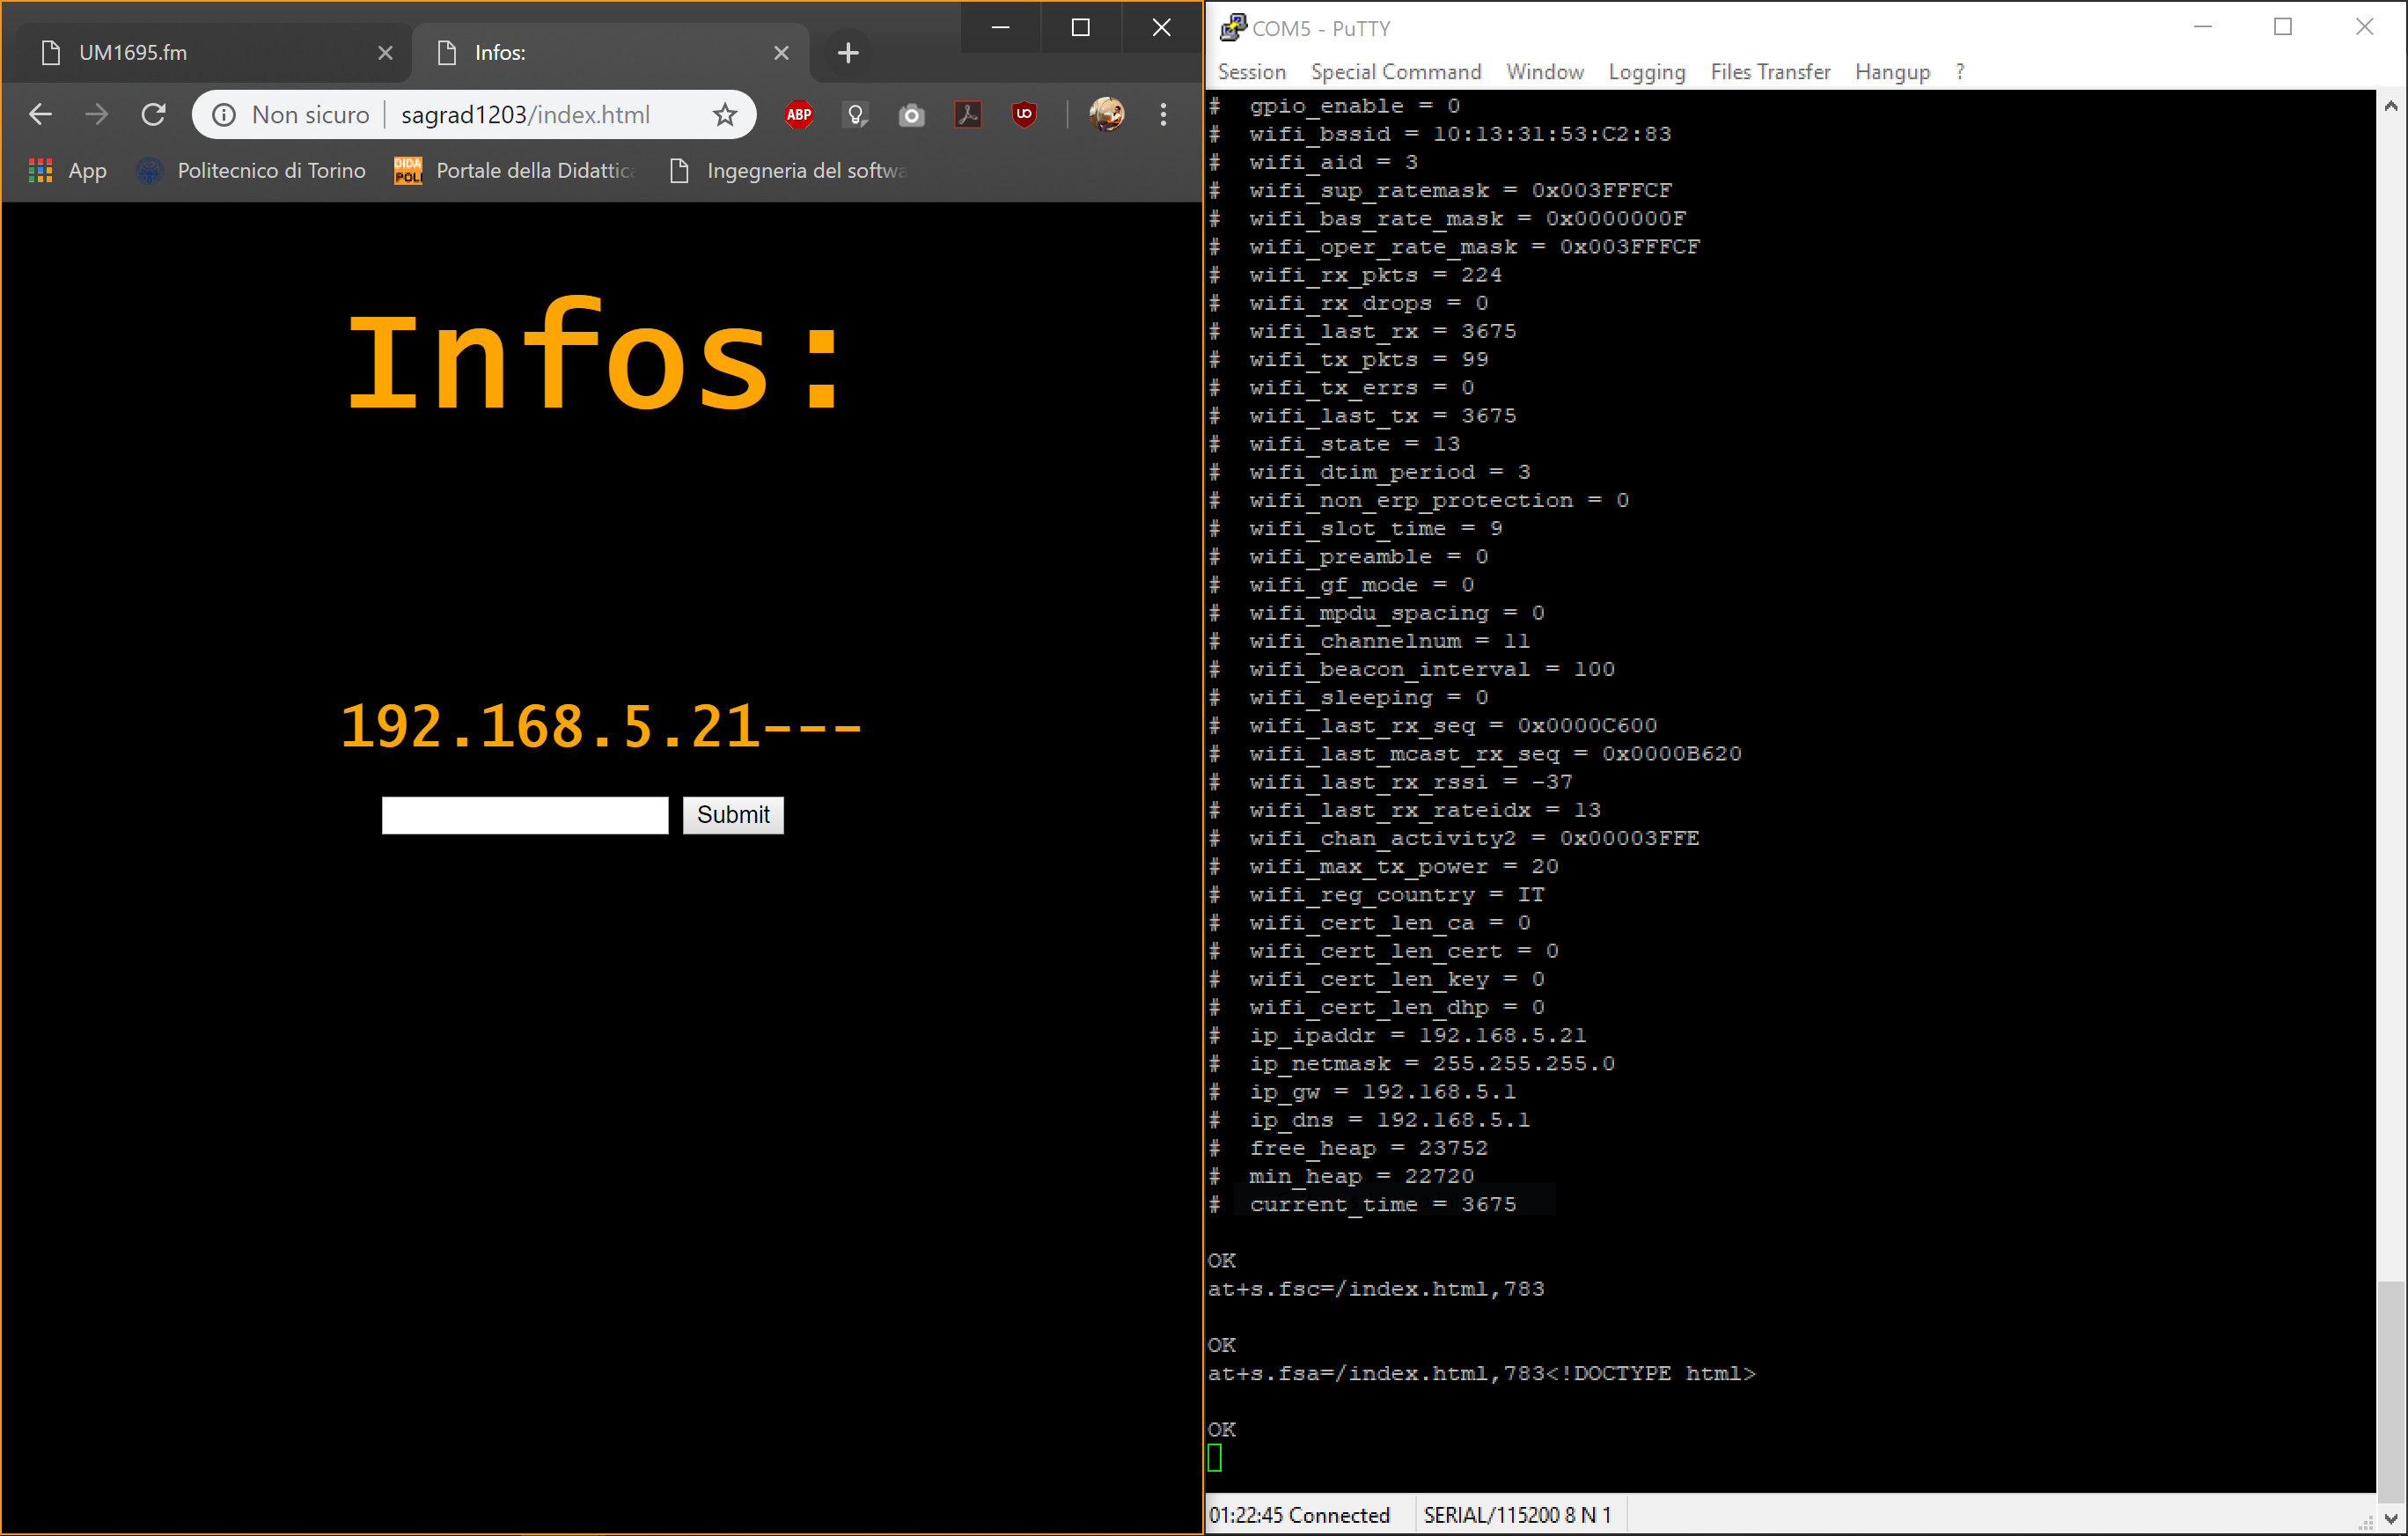
\includegraphics[width=0.8\columnwidth]{4}
\caption{IP address show web page}
\label{fig_IP}
\end{figure}
\\Note the output of the serial console command "AT+S.STS" that has to be post processed.\\
\begin{figure}[!ht]
\centering
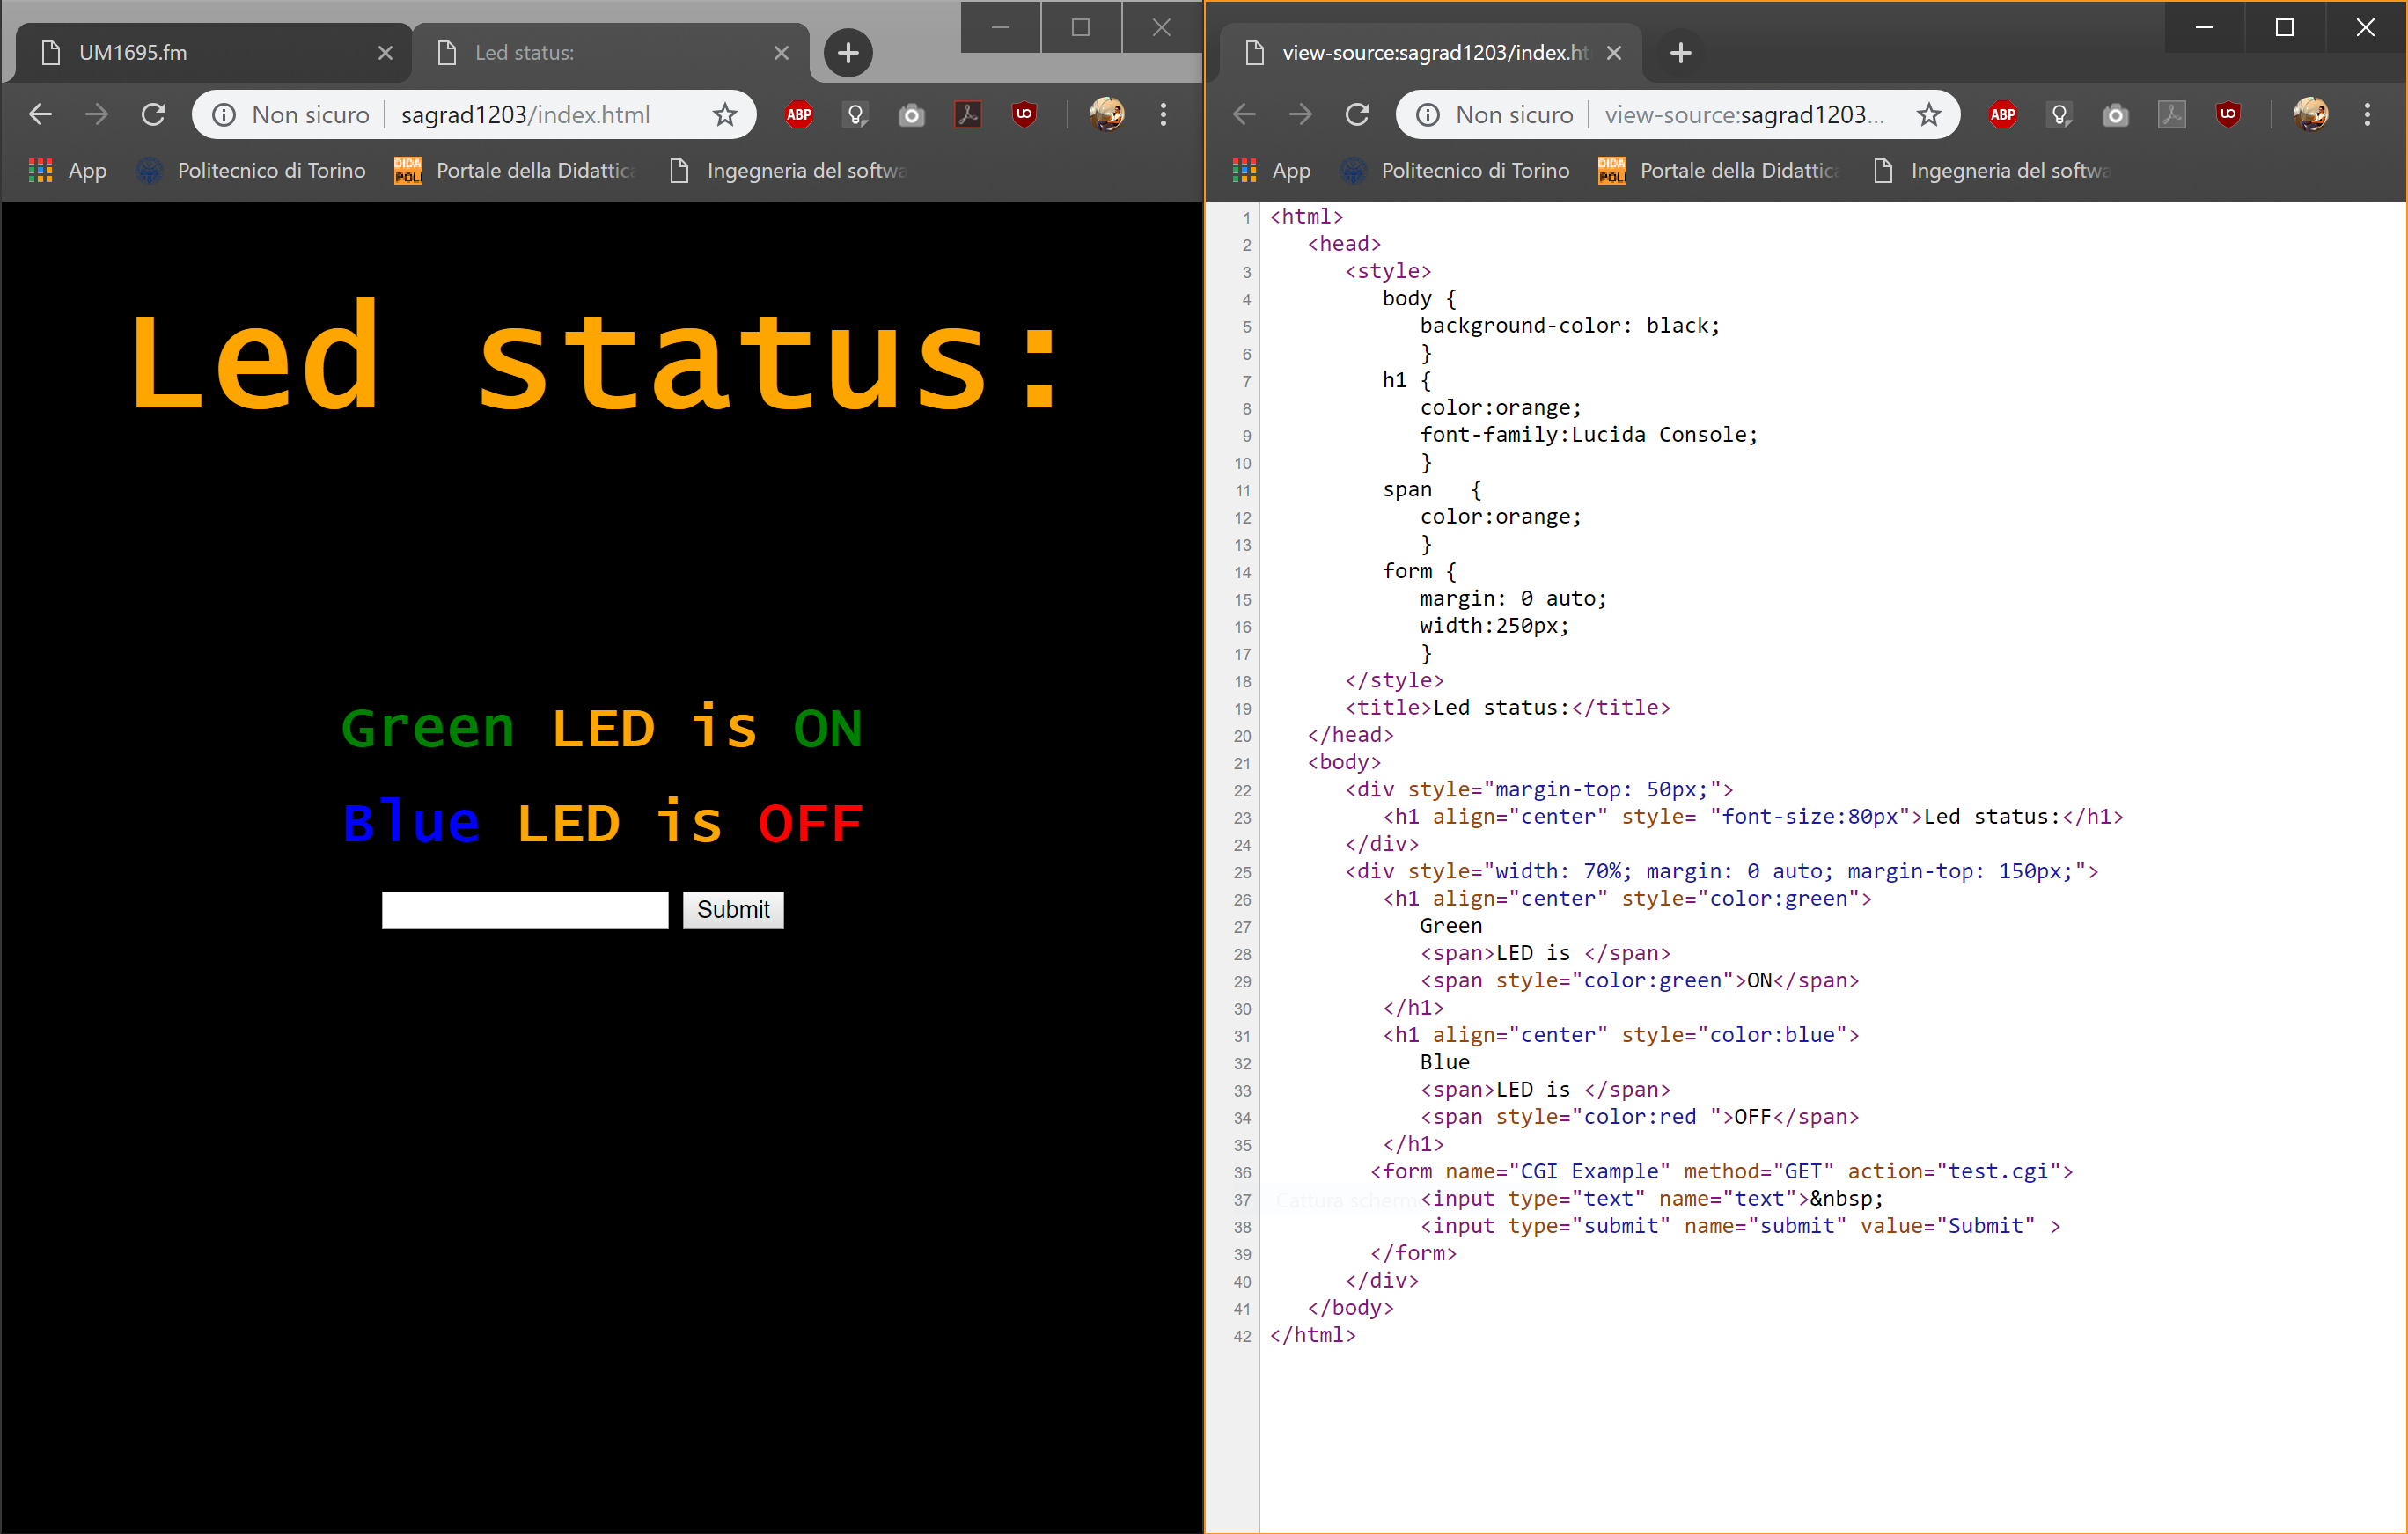
\includegraphics[width=0.8\columnwidth]{5}
\caption{well formatted HTML code retrieved}
\label{fig_HTML}
\end{figure}
\\I have decided to format the code even if formatting characters are useless for the browser and only slow the transfer but, since real bottle neck here is the UART web page transfer at 115200 baudrate, I decided to maintain formatting characters: for small web pages like this speed is not compromised.
\begin{figure}[!h]
\centering
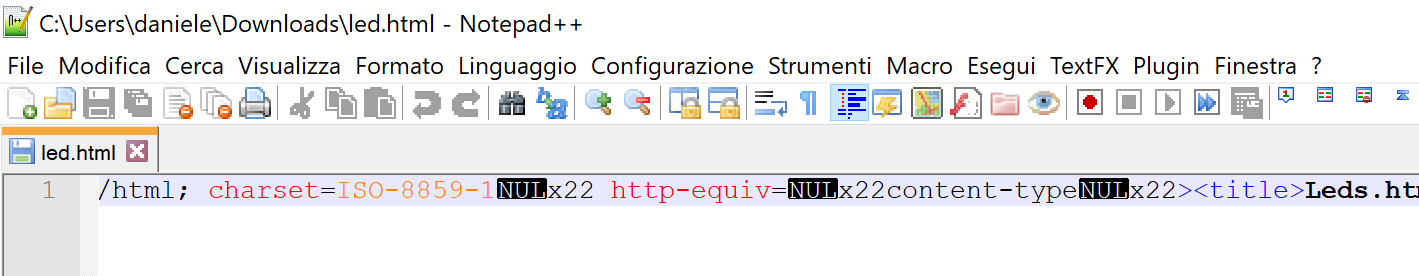
\includegraphics[width=0.8\columnwidth]{8}
\caption{led.html code retrieved}
\label{fig_led}
\end{figure}
\\Here, I finally show what I was retrieving when typing "http://sagrad1203/led.html": file was downloaded instead of being showed like I sad before and a lot of strange characters were displayed.
As I told if I had time I would also reorganized the code because, instead of putting in memory four different possible web page for each possible LED combination like it was done, I would simply memorize a single page divided in two pieces and I would concatenate them with the small piece of code to be changed during the transfer to the WiFi module like I have done for the info web page. I do not write the code here because it is too big. I would have also used \lstinline[style=CStyle]{printf();} and \lstinline[style=CStyle]{scanf();} functions I implemented in past laboratories instead of manually play with the RX buffer. That would have reduced code size and optimized it a lot .
\label{tab:template}

\section{Conclusions}
I have matched the assignment requests and, as an extra, I have fixed some template bugs restayling webpages with new HTML 5 code.

\begin{thebibliography}{1}
\bibitem{Reference_Manual}
STM32F051R8 Reference Manual (RM0091), [pdf] Available at:\\ \href{https://www.st.com/content/ccc/resource/technical/document/reference_manual/c2/f8/8a/f2/18/e6/43/96/DM00031936.pdf/files/DM00031936.pdf/jcr:content/translations/en.DM00031936.pdf}{\underline{\textcolor{blue}{Link}}}.\\Accessed on: Feb. 10, 2019.
\bibitem{User_Manual}
STM32F0DISCOVERY User Manual (UM1525), [pdf] Available at:\\ \href{https://www.st.com/content/ccc/resource/technical/document/user_manual/30/ae/6e/54/d3/b6/46/17/DM00050135.pdf/files/DM00050135.pdf/jcr:content/translations/en.DM00050135.pdf}{\underline{\textcolor{blue}{Link}}}.\\Accessed on: Feb. 10, 2019.
\bibitem{Reference_Manual_2}
SPWF01SX.11 User Manual (UM1695), [pdf] Available at:\\ \href{https://www.st.com/content/ccc/resource/technical/document/user_manual/4e/4d/c3/82/43/f1/4c/24/DM00100306.pdf/files/DM00100306.pdf/jcr:content/translations/en.DM00100306.pdf}{\underline{\textcolor{blue}{Link}}}.\\Accessed on: Feb. 10, 2019.
\end{thebibliography}

\end{document}
